\documentclass[11pt]{amsart}
\usepackage{amsmath, amssymb, amsthm}
\usepackage{todonotes}

\DeclareMathOperator*{\argmax}{argmax}
\DeclareMathOperator*{\argmin}{argmin}

\theoremstyle{definition}
\newtheorem{definition}{Definition}
\newtheorem{theorem}{Theorem}
\newtheorem{proposition}{Proposition}
\newtheorem{corollary}{Corollary}
\newtheorem{lemma}{Lemma}
\newtheorem{problem}{Problem}
\theoremstyle{remark}
\newtheorem*{remark}{Remark}
\newtheorem*{example}{Example}
\newtheorem*{solution}{Solution}

\title{Prisoner's Dilemma}
\author{Arvid Lunnemark}

\begin{document}
\maketitle

\begin{definition}
  The \textit{prisoner's dilemma} is a symmetric two-player game with two actions, cooperate ($C$) and defect ($D$), where, if player 1 plays $a$ and player 2 plays $b$, player 1 gets payoff 
  \begin{equation*}
    p(a,b) = \begin{cases}
      R &\text{if $a = C, b = C$} \\
      T &\text{if $a = D, b = C$} \\
      S &\text{if $a = C, b = D$} \\
      P &\text{if $a = D, b = D$}
    \end{cases}
  \end{equation*}
  We have $T > R > P > S$, and typically, we have the concrete values $T = 5$, $R = 3$, $P = 1$ and $S = 0$.
\end{definition}

\begin{definition}
  A \textit{strategy} is a Moore machine (finite automaton with outputs) over the input and output alphabet $\{C, D\}$, with probability $1-p$ of following the correct transition and probability $p$ of following the incorrect transition. 
\end{definition}

Note: this models an error probability in \textit{perception}. One could also think of an error probability in \textit{outcome}, but it is easy to see that the two are equivalent up to a change of the values of $R, S, T, P$.

\begin{definition}
  Suppose strategy $s_1$ plays strategy $s_2$. This defines a \textit{$s_1$-$s_2$ graph} which is a Markov chain where each node represents a pair of states $(c_1,c_2)$ where $c_1$ is a state in $s_1$ and $c_2$ is a state in $s_2$. The transition probabilities are defined in the obvious way.
\end{definition}

\begin{definition}
  Let $\pi$ be the stationary distribution achieved by starting in the start state of the \textit{$s_1$-$s_2$ graph}. The \textit{payoff} of strategy $s_1$ when played against strategy $s_2$ is \begin{equation*}
    v_{s_1}(s_2) = \sum \pi_{c_1, c_2} \cdot p(c_1, c_2).
  \end{equation*}
\end{definition}

Note: The graph might be periodic in which case we we will not get a stationary distribution. I need to think about this special case but my intuition is that it shouldn't matter.

\begin{definition}
  A \textit{population} of strategies $P = (S, f)$ is a set $S$ of strategies and a function $f : S \to (0,1]$ such that $\sum_{s \in S} f(s) = 1$, representing the frequency of each strategy in the population.
\end{definition}

\begin{definition}
  The \textit{fitness} of a strategy $s$ in a population $P = (S, f)$ is \begin{equation*}
    F(s) = \sum_{s' \in S} f(s') v_s(s').
  \end{equation*}
\end{definition}

\begin{definition}
  A strategy $s_1$ is \textit{$\epsilon$-invadable} if there exists a strategy $s_2$ such that in all populations $P$ with $S = \{s_1,s_2\}$ and $f(s_2) \geq \epsilon$, we have \begin{equation}
    \label{fitnesscond}
    F(s_2) > F(s_1)
  \end{equation}
\end{definition}

\begin{definition}
  A strategy $s_1$ is \textit{evolutionary stable} if there exists an $\alpha \in (0,1)$ such that for all $\epsilon < \alpha$, $s_1$ is not $\epsilon$-invadable.
\end{definition}

Note: it is easy to see that this is just equivalent to saying that there exists some $\epsilon$ for which $s_1$ is not $\epsilon$-invadable.

\begin{theorem}
  Suppose $s_1$ is evolutionary stable. Then $v_{s_1}(s_1) \geq \frac{S + T}{2}$.
\end{theorem}

\begin{theorem}
  Suppose $s_1$ is evolutionary stable as $p$ goes to 0 (i.e., that it is evolutionary stable if condition \ref{fitnesscond} is replaced by $\lim_{p \to 0} (F (s_2)-F(s_1)) > 0$). Then $v_{s_1}(s_1) = R$. In other words, $s_1$ is utilitarian.
\end{theorem}

\begin{theorem}
  The Pavlov strategy, displayed in Figure ??, is evolutionary stable as $p$ goes to 0.
\end{theorem}

\begin{remark}
  TFT, displayed in Figure ??, is not evolutionary stable as $p$ goes to 0. It has the stationary distribution $(1/4,1/4,1/4,1/4)$ which is smaller than $R$.
\end{remark}


\begin{figure}
  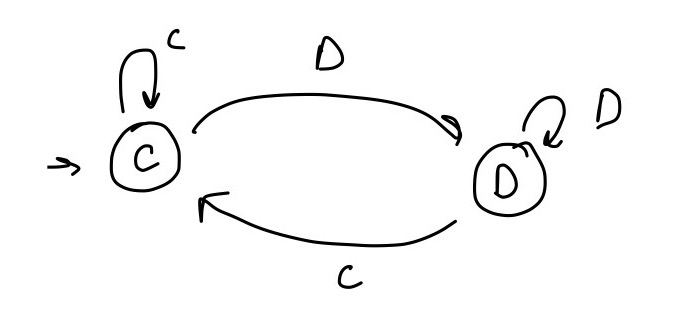
\includegraphics[width=4cm]{tft.jpg}
  \centering
  \caption{TFT.}
  \end{figure}
\begin{figure}
  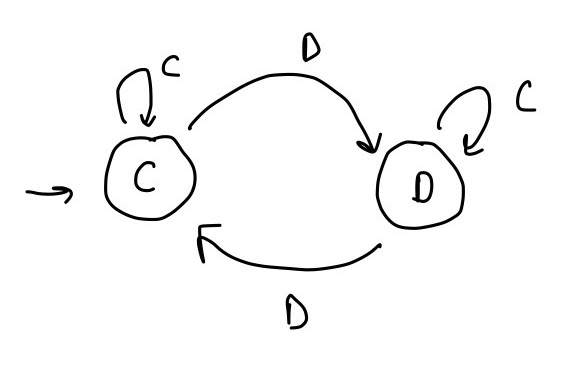
\includegraphics[width=4cm]{pavlov.jpg}
  \centering
  \caption{Pavlov.}
  \end{figure}


\end{document}